% Document class and two-column conversion
\documentclass{report}
% dimensions of paper and relative text positioning
\usepackage[a4paper,top=2cm,bottom=2cm,left=2cm,right=2cm]{geometry}
% math symbols
\usepackage{amsmath}
\usepackage{amssymb}
% package for including URLs
\usepackage{url}
% Required for including images
\usepackage{graphicx}
\usepackage{float} % Required for specifying the exact location of a figure

% enable writing in greek
\usepackage[greek,english]{babel}
\usepackage[utf8]{inputenc}
%\usepackage[LGR]{fontenc}

\setlength{\parindent}{0pt} % Removes all indentation from paragraphs

% Start of the document
\begin{document}

% Set the language to greek
\selectlanguage{greek}

% Title page
\title{\Huge \bfseries Τεχνικές Βελτιστοποίησης \\ Τρίτο Παραδοτέο} %\Huge and \bfseries are used to make the title bigger and bold
\author{Παπαδάκης Κωνσταντίνος Φώτιος\vspace{0.5cm} \\  ΑΕΜ:10371} % \vspace{0.5cm} is used to add some vertical space between the author and the AEM
\date{\today}
% prints the title, author and date on a separate page
\maketitle

% Table of contents page
\tableofcontents

% General introduction
\chapter{Εισαγωγή}
\section{Γενικά}
Η συνάρτηση που θα εξετάσουμε στο τρίτο παραδοτέο είναι η εξής:
$$ f: \mathbb{R}^2 \to \mathbb{R},\; f(x) = \frac{1}{3} x_1^2 + 3x_2^2,\; x = [x_1 x_2]^T$$



% Steepest Descent: Various constant steps
\chapter{Θέμα 1}
\section{Εκφώνηση}
Να χρησιμοποιηθεί η Μέθοδος Μέγιστης Καθόδου (προηγούμενη εργασία) με ακρίβεια $\epsilon =
0.001$ και βήμα:
\begin{itemize}
    \item i) $\gamma_k$ = 0.1
    \item ii) $\gamma_k$ = 0.3
    \item iii) $\gamma_k$ = 3
    \item iv) $\gamma_k$ = 5
\end{itemize}
και οποιοδήποτε αρχικό σημείο εκκίνησης διαφορετικό του $(0,0)$. Τι παρατηρείτε
\selectlanguage{english};\selectlanguage{greek} Να αποδειχθούν τα αποτελέσματα αυτά 
με μαθηματική αυστηρότητα.
\section{Λύση}
Επέλεξα το σημείο εκκίνησης $(-1,1)$ ως το πιο ενδιαφέρον σημείο που εξετάσαμε στο δεύτερο παραδοτέο.
Το διάγραμμα που προκύπτει από την εκτέλεση του αλγορίθμου Μέγιστης Καθόδου με διάφορα σταθερά βήματα είναι
το εξής:
\begin{figure}[H]
    \centering
    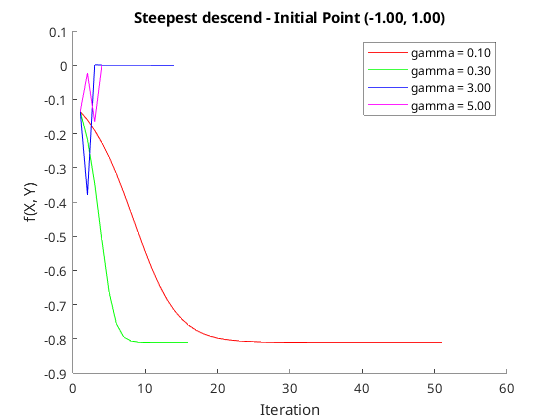
\includegraphics[width=0.8\textwidth]{media/thema1.png}
    \caption{Διάγραμμα Μέγιστης Καθόδου με διάφορα σταθερά βήματα}
\end{figure}

\subsection{Μαθηματική Απόδειξη}


\subsection{Εισαγωγή Περιορισμών}
Θεωρήστε τώρα τους περιορισμούς:
$$-10 <= x_1 <= 5$$  
\begin{center}
    και
\end{center}
$$-8 <= x_2 <= 12$$

% 
\chapter{Θέμα 2}
\section{Εκφώνηση}
Να χρησιμοποιηθεί η Μέθοδος Μέγιστης Καθόδου με Προβολή, με $s_k = 5$, $\gamma_k = 0.5$,
σημείο εκκίνησης το $(5, -5)$ και ακρίβεια $\epsilon = 0.01$. Τι παρατηρείτε σε σχέση με το 
Θέμα 1\selectlanguage{english};\selectlanguage{greek}
\section{Λύση}
\section{Λύση}


% 
\chapter{Θέμα 3}
\section{Εκφώνηση}
Να χρησιμοποιηθεί η Μέθοδος Μέγιστης Καθόδου με Προβολή, με $s_k = 15$, $\gamma_k = 0.1$,
σημείο εκκίνησης το $(-5,10)$ και ακρίβεια $\epsilon = 0.01$. Τι παρατηρείτε σε σχέση με τα Θέματα 1 
και 2\selectlanguage{english};\selectlanguage{greek}
\section{Λύση} Προτείνετε έναν απλό πρακτικό τρόπο ώστε η μέθοδος να συγκλίνει στο ελάχιστο.
\section{Λύση}


% 
\chapter{Θέμα 4}
\section{Εκφώνηση}
Να χρησιμοποιηθεί η Μέθοδος Μέγιστης Καθόδου με Προβολή, με $s_k = 0.1$, $\gamma_k = 0.2$,
σημείο εκκίνησης το $(8, -10)$ και ακρίβεια $\epsilon = 0.01$. Σε αυτή την περίπτωση, έχουμε εκ των
προτέρων κάποια πληροφορία σχετικά με την σύγκλιση του αλγορίθμου\selectlanguage{english};
\selectlanguage{greek}
\section{Λύση} Να γίνει η εκτέλεση του
αλγορίθμου. Τι παρατηρείτε\selectlanguage{english};\selectlanguage{greek}
\section{Λύση}

% Comparison
\chapter{Ανάλυση αποτελεσμάτων}

\section{Σχόλια}


% Bibliography
\nocite{*} % Include all references in the bibliography, even if they are not cited in the report
\bibliographystyle{plain}
\bibliography{references/references} % We have to include the references somewhere in the report for them to show here if we don't use (\nocite{*})
\addcontentsline{toc}{chapter}{\bibname} % Add the bibliography to the table of contents

% End of the document
\end{document}